\chapter{Data acquisition software}
\label{chapter:dqm4hep}

\epigraph{Before software can be reusable \\it first has to be usable.}{Ralph Johnson}

Data acquisition is a critical component of all particle physics experiments across all stages of technological readiness, from the very beginning of hardware testing in tabletop experiments to full-scale international experiments like the Large Hadron Collider. 

In the modern era of particle physics, the interplay of hardware and software at minscule timescales drives everything, and almost all results are highly dependent upon the speed and efficiency of the electronics and computer systems that extract data from the detectors. A massive quantity of work goes into creating, testing and optimising the systems that will acquire, process, sort and transport data before it is ever seen by the physicist operating the experiment.

Of particular interest in this thesis is the data acquisition software during the development phase, where individual detector subcomponents are undergoing prototyping and testing. These development and iteration cycles are tied closely to testbeam facillities such as the Super Proton Synchrotron (SPS) at CERN and the DESY II synchrotron at DESY. At this point in the development cycle, the detectors are beginning to take shape and this is where data acquisition (or DAQ) becomes an important consideration. 

In addition to this, the data acquisition solutions used during the testbeam phase of detector development is likely to inform the final data acquisition solution, either directly by evolving into the final software, or indirectly by identifying and evaluating the particular features or challenges of the subdetector components that the software must take into account or accommodate.

During this stage, each individual detector component -- such as a vertex tracker or hadronic calorimeter -- will be developed by small teams, and the natural tendency is for each of these groups to set their own standards and develop their own tools, prioritising the features that are important to their specific case. However, in the past this approach has generated a variety of \textit{ad hoc} solutions for testbeam software, many of which cannot be applied outside of their original scope. The also results in wasted effort and time, as different teams implement the same solutions anew for each subdetector.

One of the aims of the AIDA-2020 project is to improve this situation by developing generic and reusable software tools for testbeams and particle physics experiments.

\subsubsection{The AIDA-2020 project}
The AIDA-2020 project is an EU-funded research programme for developing infrastructure and technologies for particle physics detector development and testing, comprising 24 member countries and lead by CERN.

The overarching goal of the project is to develop common infrastructures and tools for physics testbeams, and software is one such important tool. By creating a suite of tools that are designed with a variety of uses in mind, the amount of effort and development time necessary to plan and implement data acquisition and monitoring setups can be significantly reduced or eliminated, speeding up the planning and deployment of physics testbeams. This allows more science to be done faster. The two tools within AIDA-2020 that facillitate this are EUDAQ and DQM4hep, discussed in more detail below.

\section{Overview of DQM4hep}
Data Quality Monitoring for High-Energy Physics (abbreviated DQM4hep) is an online monitoring and data quality monitoring framework developed for physics testbeams for high-energy and particle physics. It is designed to be able to fulfil the requirements of monitoring for physics testbeams in a generic way. The framework is written in the C++11 standard and can run on any Linux distribution. The only requirements for installation are a compiler compliant with the C++11 standard, cmake 3.4 or higher, and ROOT 6. All other dependencies are downloaded and compiled automatically during installation. 

The two core principles of DQM4hep are genericity and modularity. The core of the system is based on a plugin system that allows shared libraries to be loaded and hook classes for further use \cite{aida2020-milestone-dqm4hep}. 

This structure allows for independent components of the framework to be used, not used, or exchanged, by isolating each function of the program into specific and independent processes. The components that are specific to particular users are written by those users, and the rest of the framework then handles packaging this information in a useful way and networking to transmit it to where it is needed, meaning that the user does not have to worry about the mechanics of data storage, serialisation or transmission. 

The experiment-specific components have to be written by the user, but these components use standard C++ code with a few DQM4hep-specific functions to handle their integration into the framework, making them easy to understand for users who already have experience coding in C++. This also means that the framework is capable of working with any data format that can packed into, decoded from, and accessed with normal C++ methods, including those that can be loaded from external libraries. This results in a framework that is able to deal with any kind of data, including user-defined data types, making it more flexible, portable and easily reusable.

\subsection{Architecture}
DQM4HEP is designed with genericness as its core paradigm, using processes and algorithms that are independent of data type. The ability to run multiple instances of each process of the framework is also key to its flexibility, allowing users to, for example, separate sub-detector data from data that has undergone event building, operate in online or offline modes, or distribute the computational load of the analysis over several networked computers.

The generic nature of the framework lies in two core features:
\begin{itemize}
	\item The Event Data Model abstraction allows the user to define the type and structure of an event and how serialisation should be handled.
	\item The plugin system allows the inclusion of any user-defined classes via external libraries, such as to select the serialisation process, online analysis, etc.
\end{itemize}

The plugin system for end-users consists of four different types of plugins: analysis modules, standalone modules, file reader plugins, and file streamer plugins. Each of these will be discussed in-depth in the sections below.

A diagrammatical representation of the overall structure of the framework can be seen in Fig. \ref{figure:daq/dqm4hep/architecture}.

\subsubsection{Analysis modules}
Analysis modules recieve events from the data aquisition system, processing the data according to a user-specified procedure to create ROOT TObjects like histograms, graphs, plots, etc. The analysis module then handles encapsulating these objects as monitor elements, and sending them to the rest of the framework for display and storage. 

An analysis module is specific to one use case, and is intended to be written by the user with their data format and processing needs in mind. However, the framework provides both templates and examples for how to write an analysis module. 

An example of the structure of the framework utilising an analysis module can be seen in Fig. \ref{figure:daq/dqm4hep/analysis-module}.

\subsubsection{Standalone modules}
Standalone modules are identical in form to analysis modules described above. The distinction is that a standalone module does not operate on data coming from the data aquisition device. One of the intended and most common usages of standalone modules is as a slow control, taking data from monitoring sensors on the device rather than data, to report on the condition of the hardware. Standalone modules could also be used to \emph{generate} data, if needed, acting as a programmed signal generator or random number generator. 

An example of the structure of the framework utilising a standalone module can be seen in Fig. \ref{figure:daq/dqm4hep/standalone-module}.

\subsubsection{File reader plugins}
A file reader is a type of plugin that reads a file from the disk and packs it into a data structure necessary for usage within DQM4hep. They are used primarily for offline monitoring or data processing. File readers can be made for any kind of file, provided the user understands the data structure. There are existing examples of file readers for data stored as binary, plain text, LCIO files, and ROOT TTrees. 

An example of the structure of the framework utilising a file reader plugin can be seen in Fig. \ref{figure:daq/dqm4hep/file-reader}.

\subsubsection{File streamer plugins}
A file streamer is a type of plugin that reads data from a stream and packs it into a data structure necessary for usage within DQM4hep. They are for receiving data from a data acquisition device for online monitoring. File streamers can be made for any kind of data stream, provided the user understands the data structure. File streamers are considered the ``default'' in DQM4hep.

\begin{figure}[h]
	\centering
	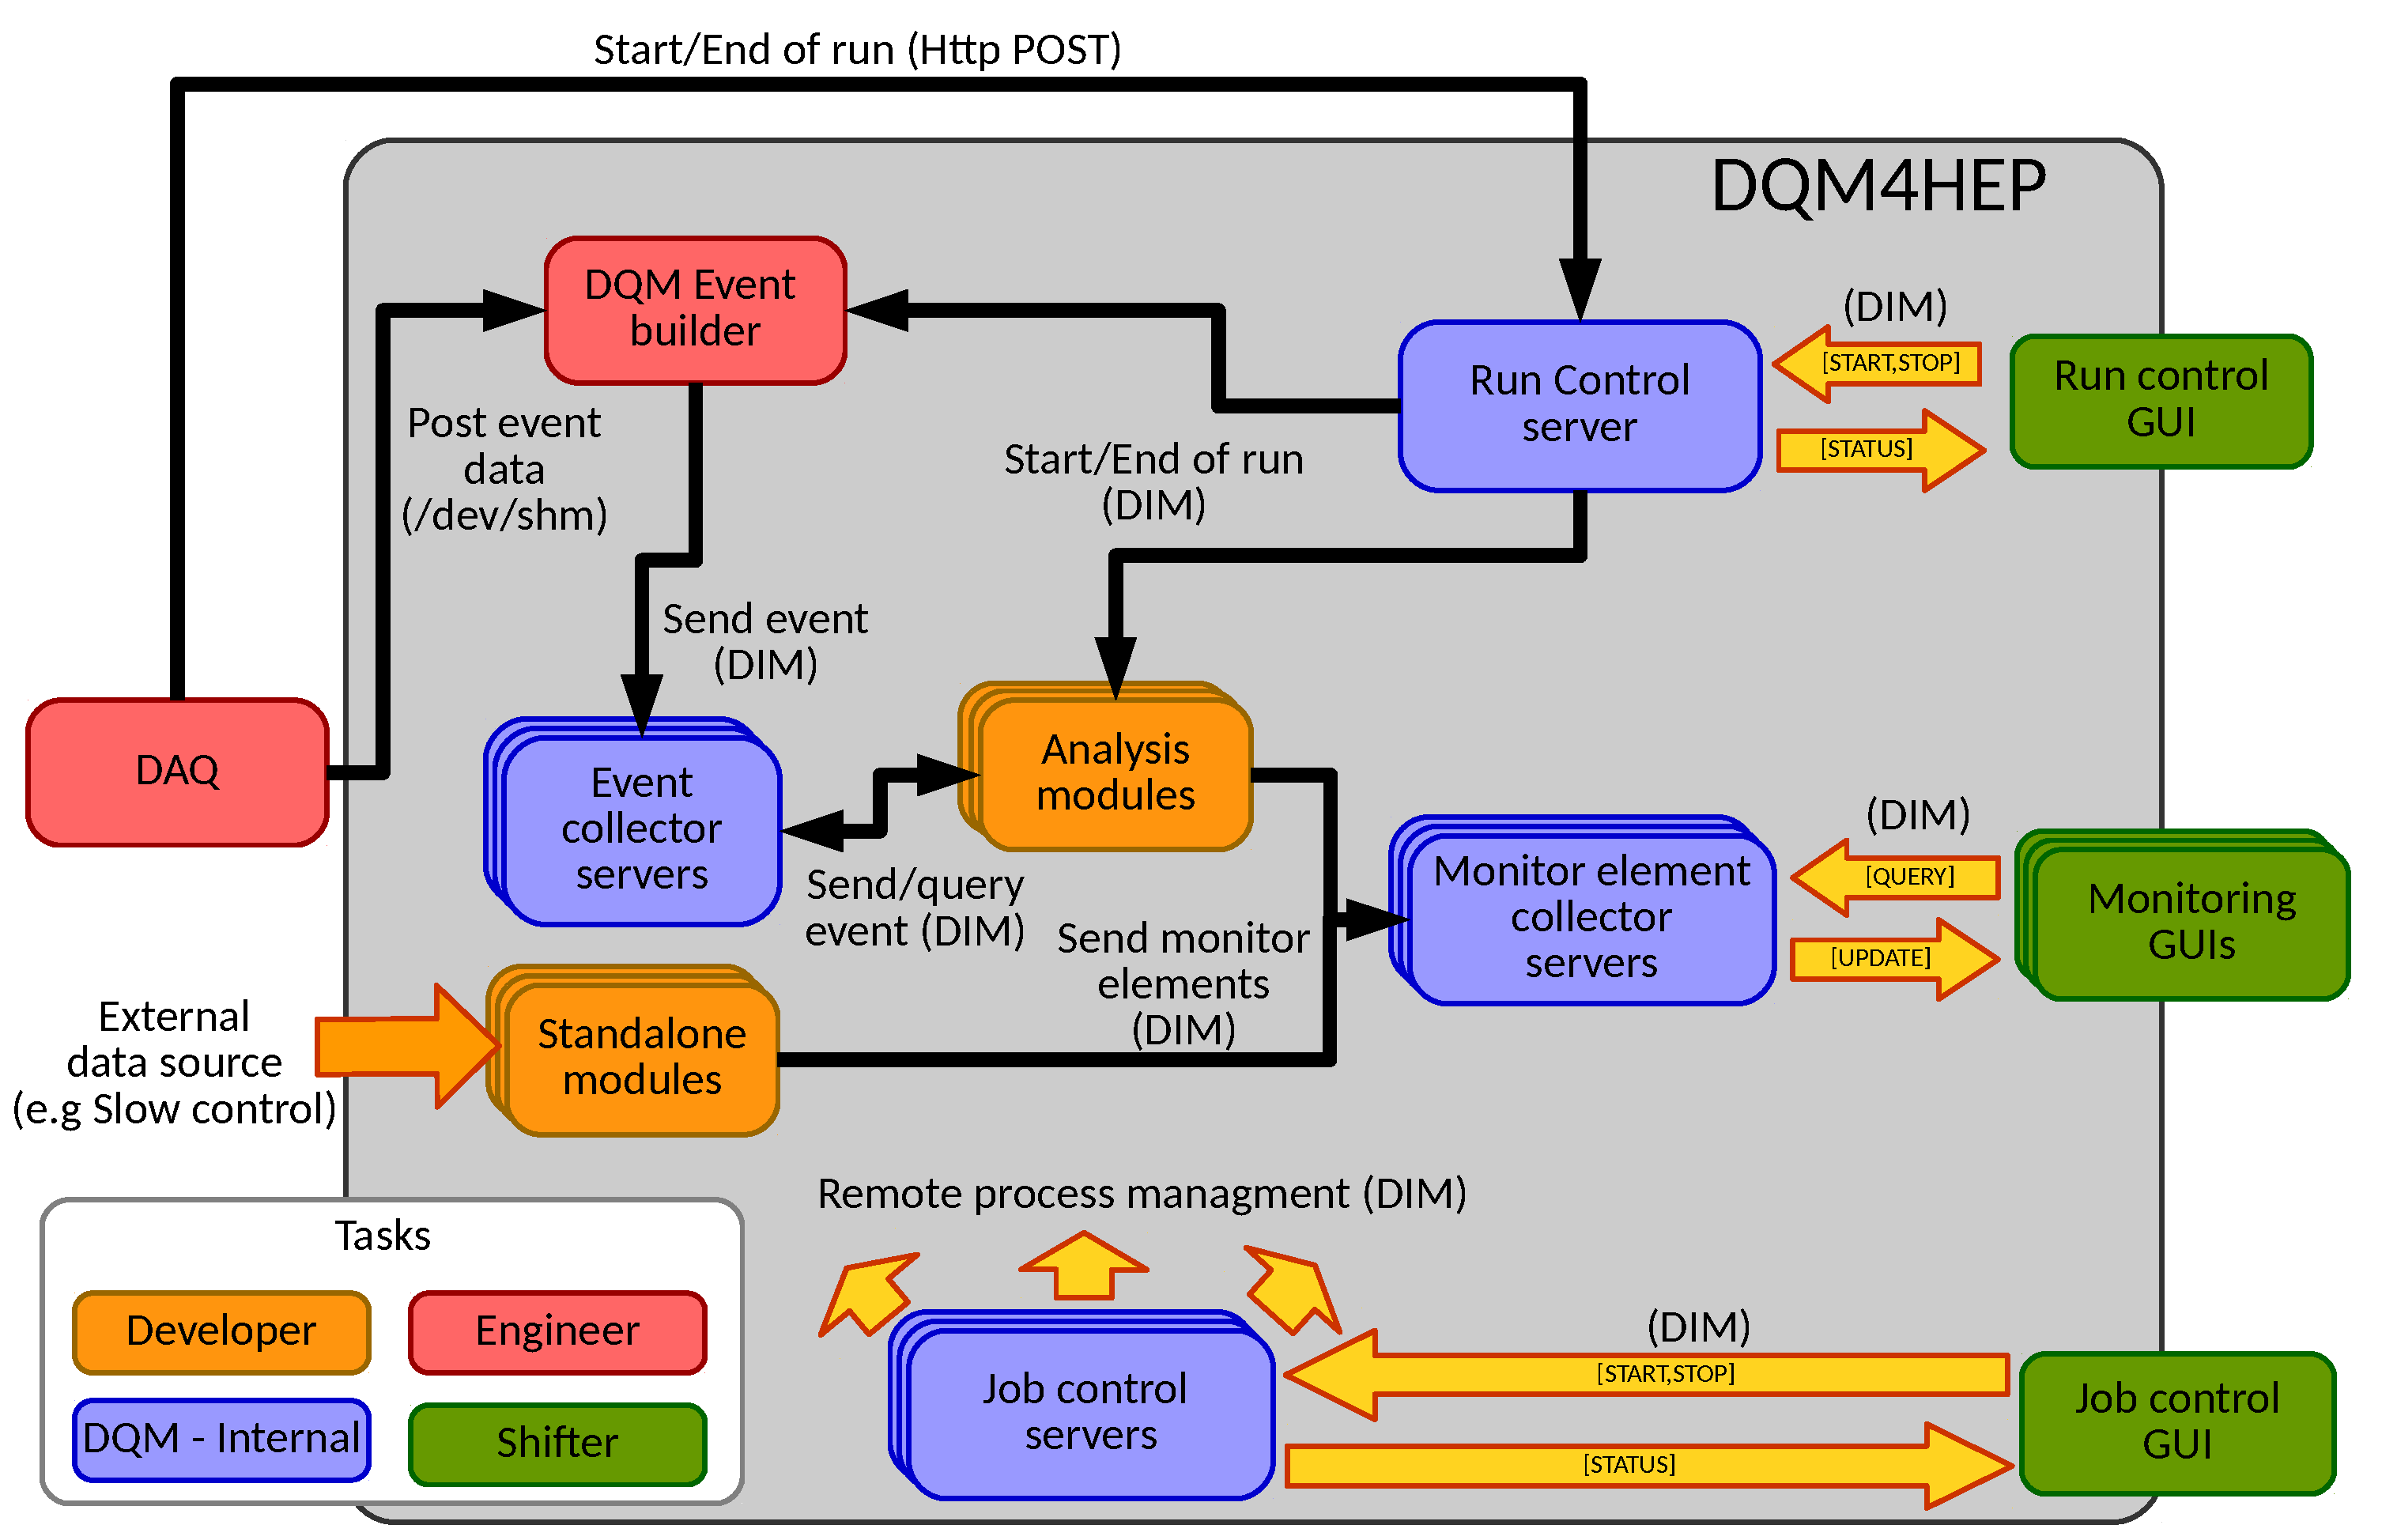
\includegraphics[width=0.95\textwidth]{../Pictures/GlobalArchitectureDiagram.pdf}
	\caption{The global online architecture of DQM4hep. Each block is colour-coded to show which operator of the testbeam is responsible for the process.}
	\label{figure:daq/dqm4hep/architecture}
\end{figure}

\begin{figure}
	\centering
	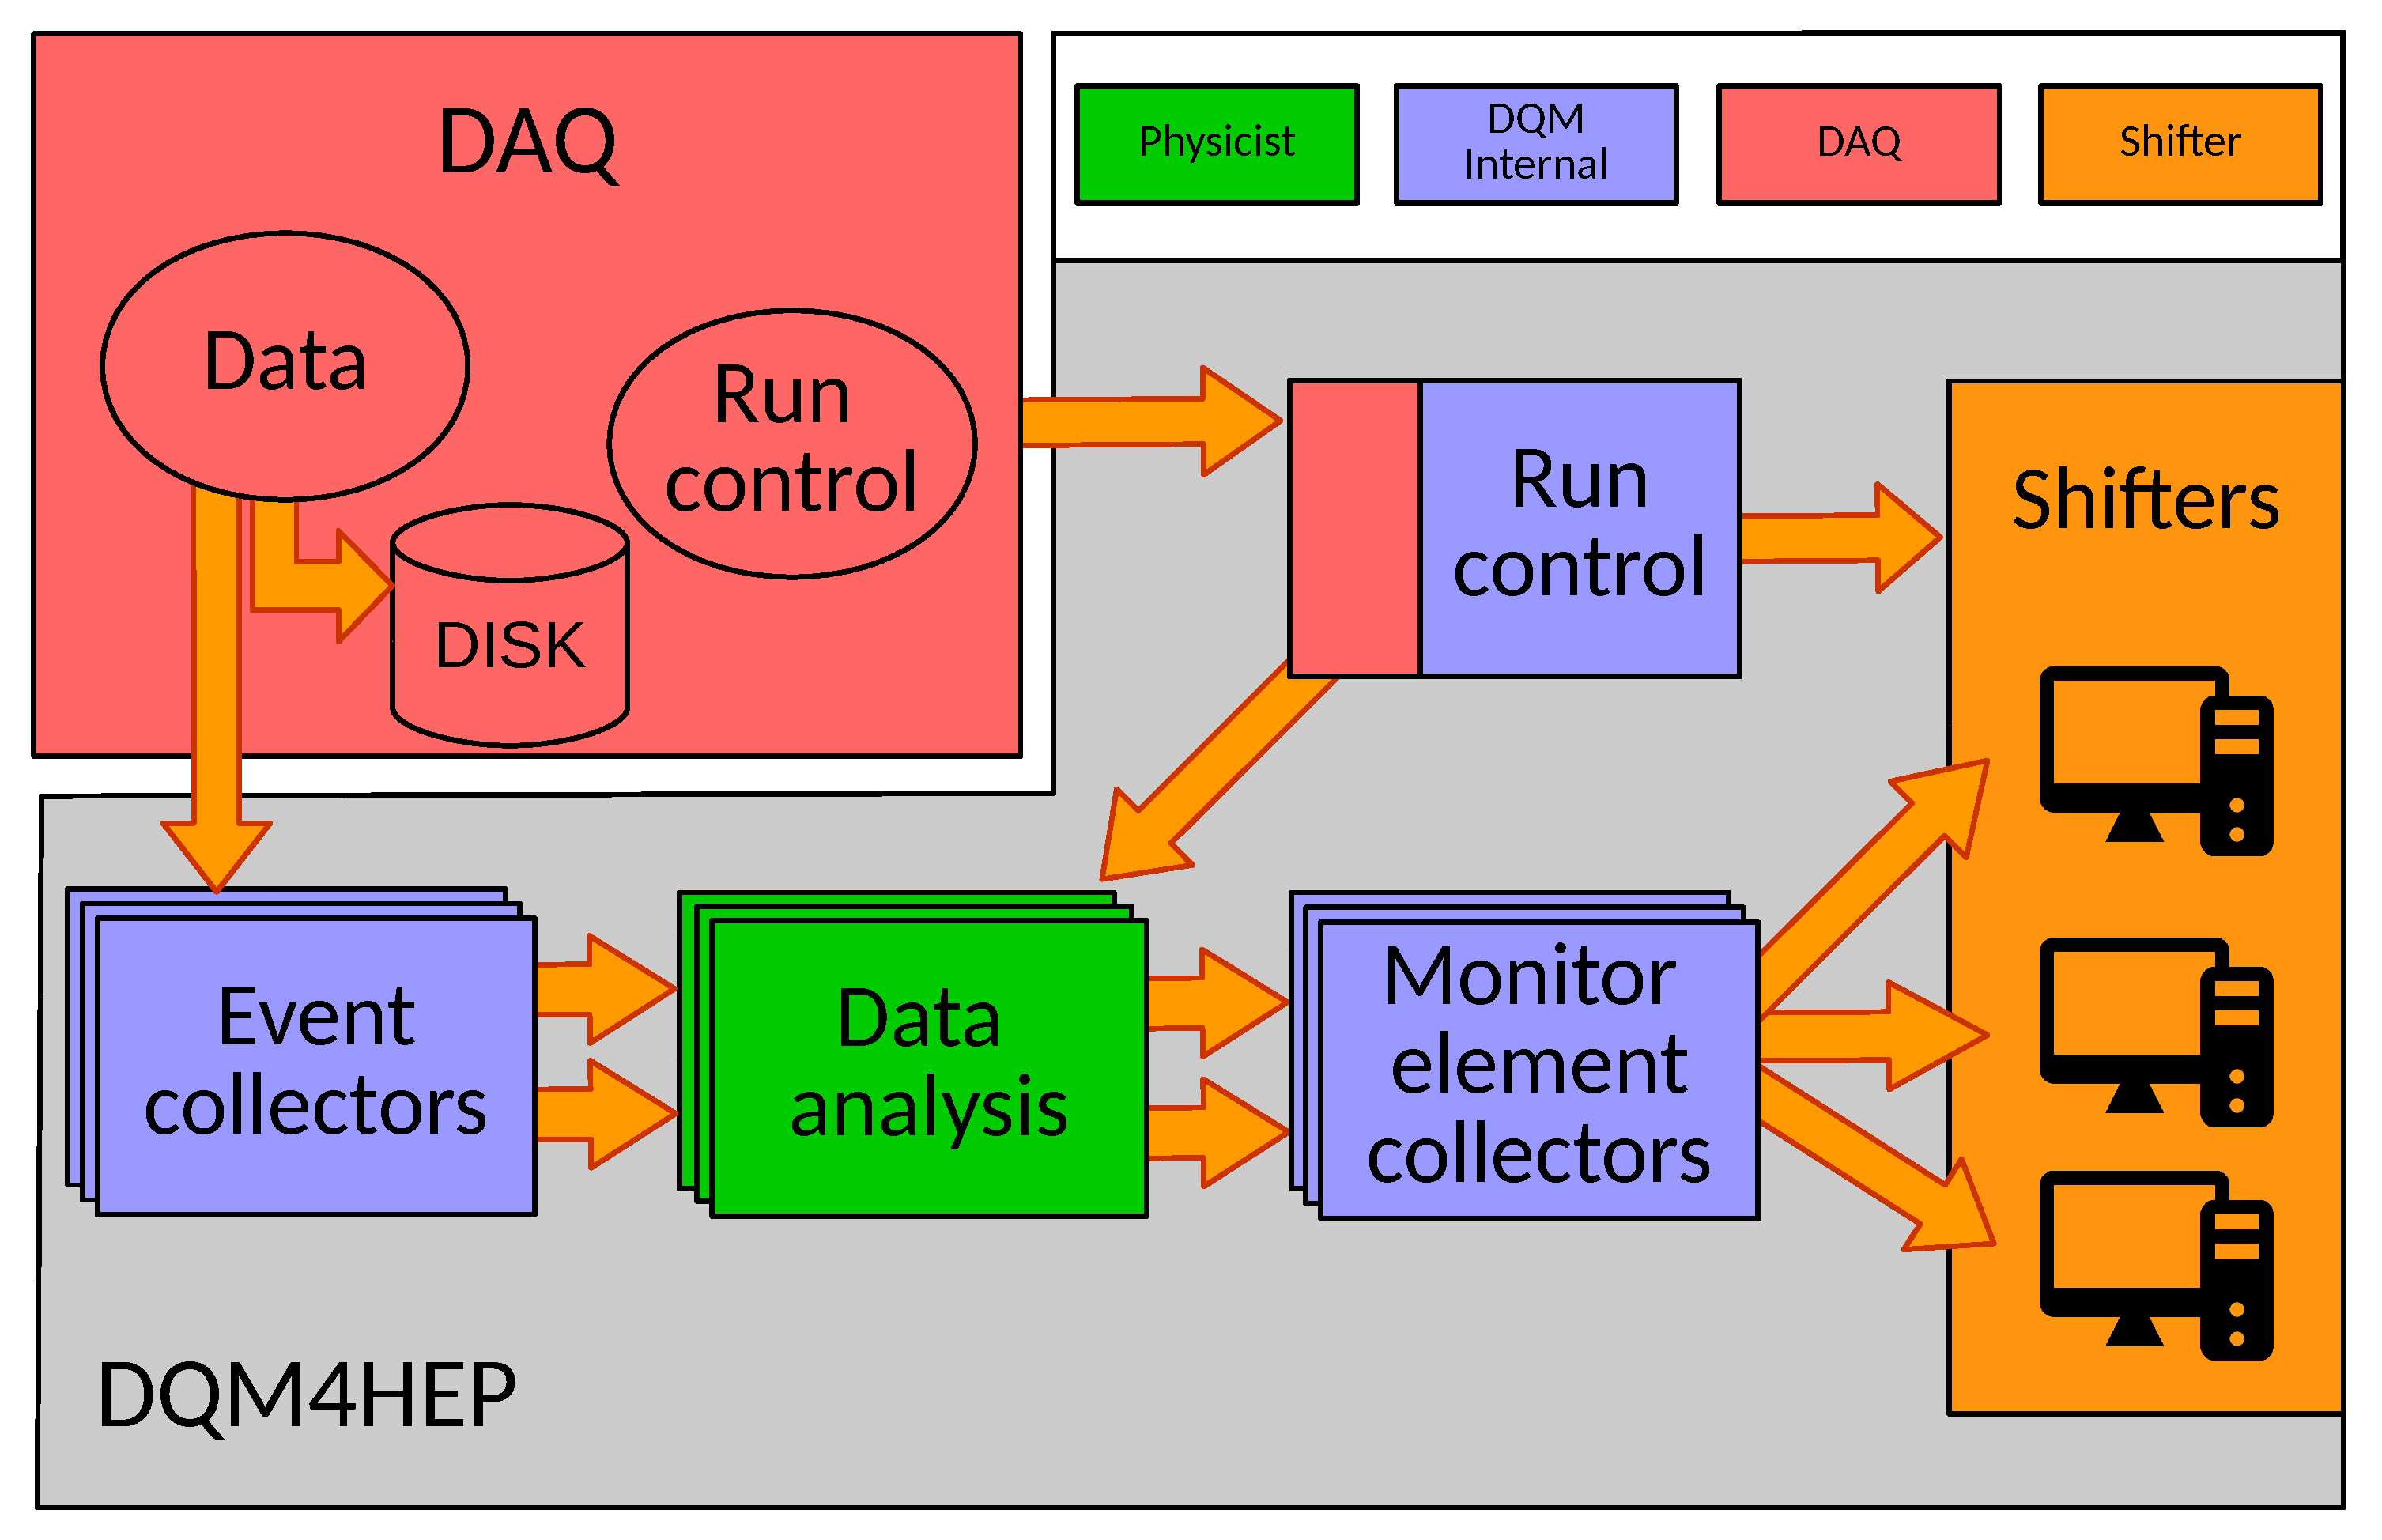
\includegraphics[width=0.95\textwidth]{../Pictures/AnalysisModuleArchitecture.pdf}
	\caption{The structure of running DQM4hep online using an analysis module.}
	\label{figure:daq/dqm4hep/analysis-module}
\end{figure}

\begin{figure}
	\centering
	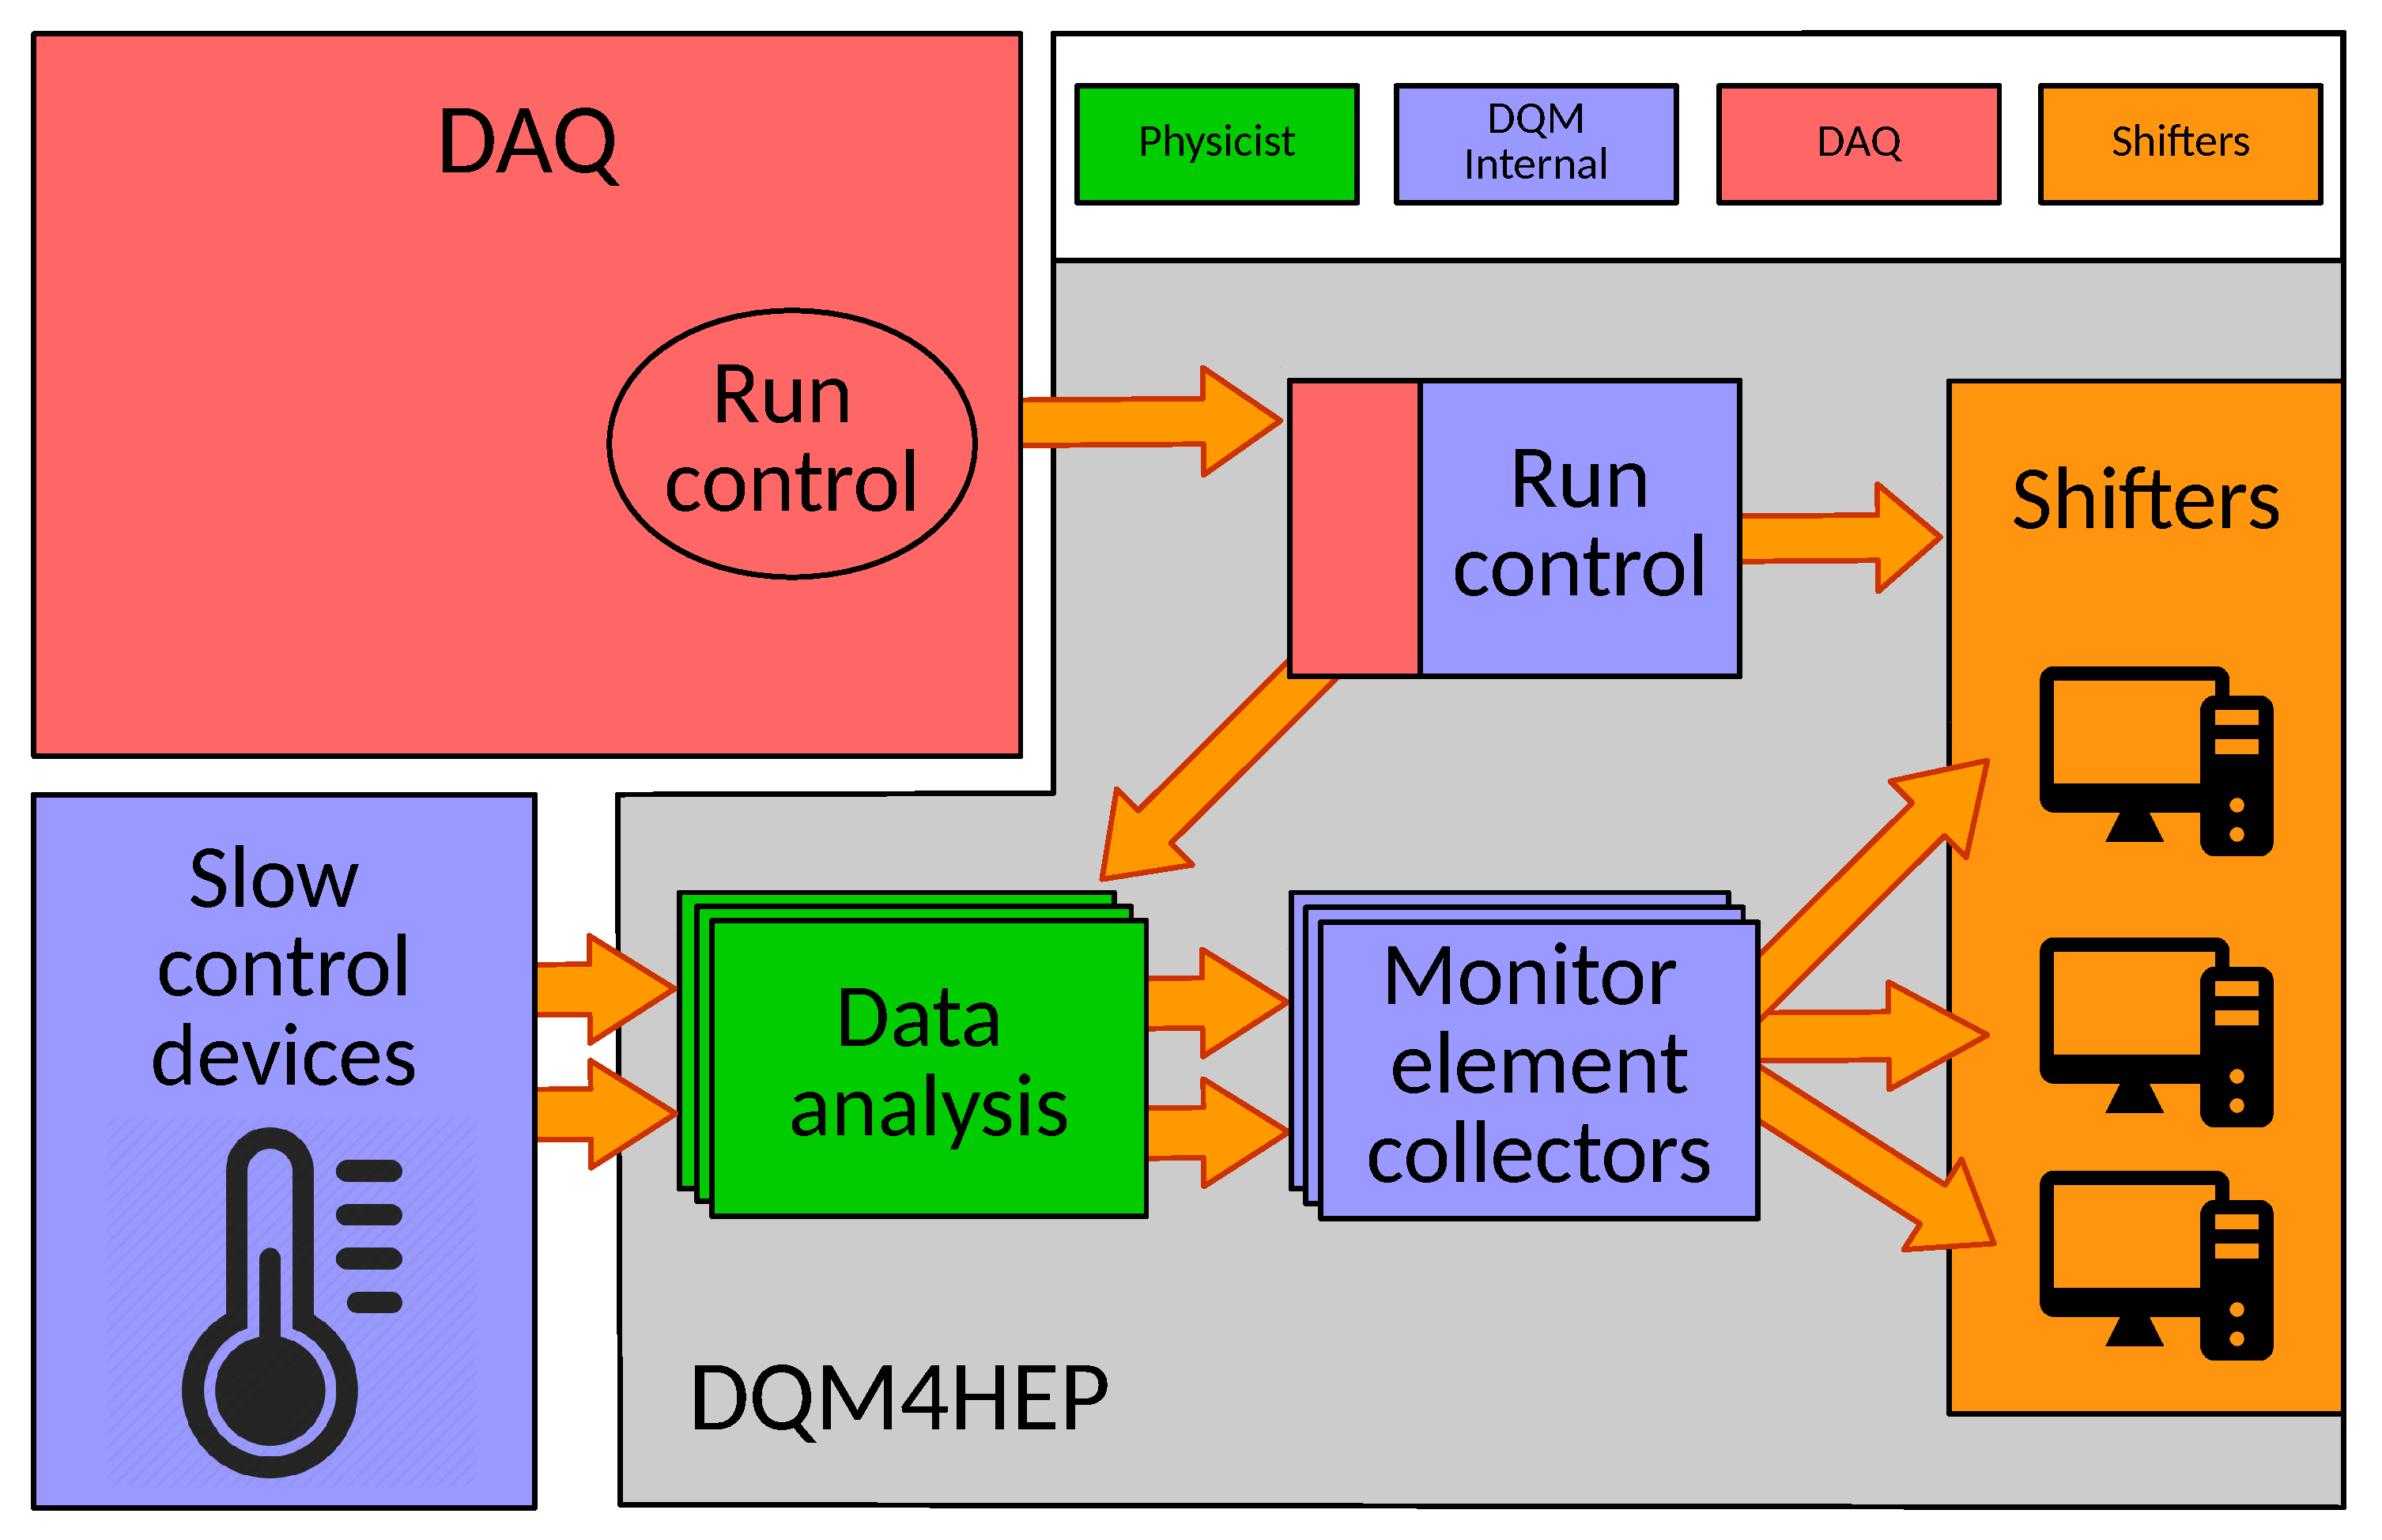
\includegraphics[width=0.95\textwidth]{../Pictures/StandaloneModuleArchitecture.pdf}
	\caption{The structure of running DQM4hep online using a stand alone module.}
	\label{figure:daq/dqm4hep/standalone-module}
\end{figure}

\begin{figure}
	\centering
	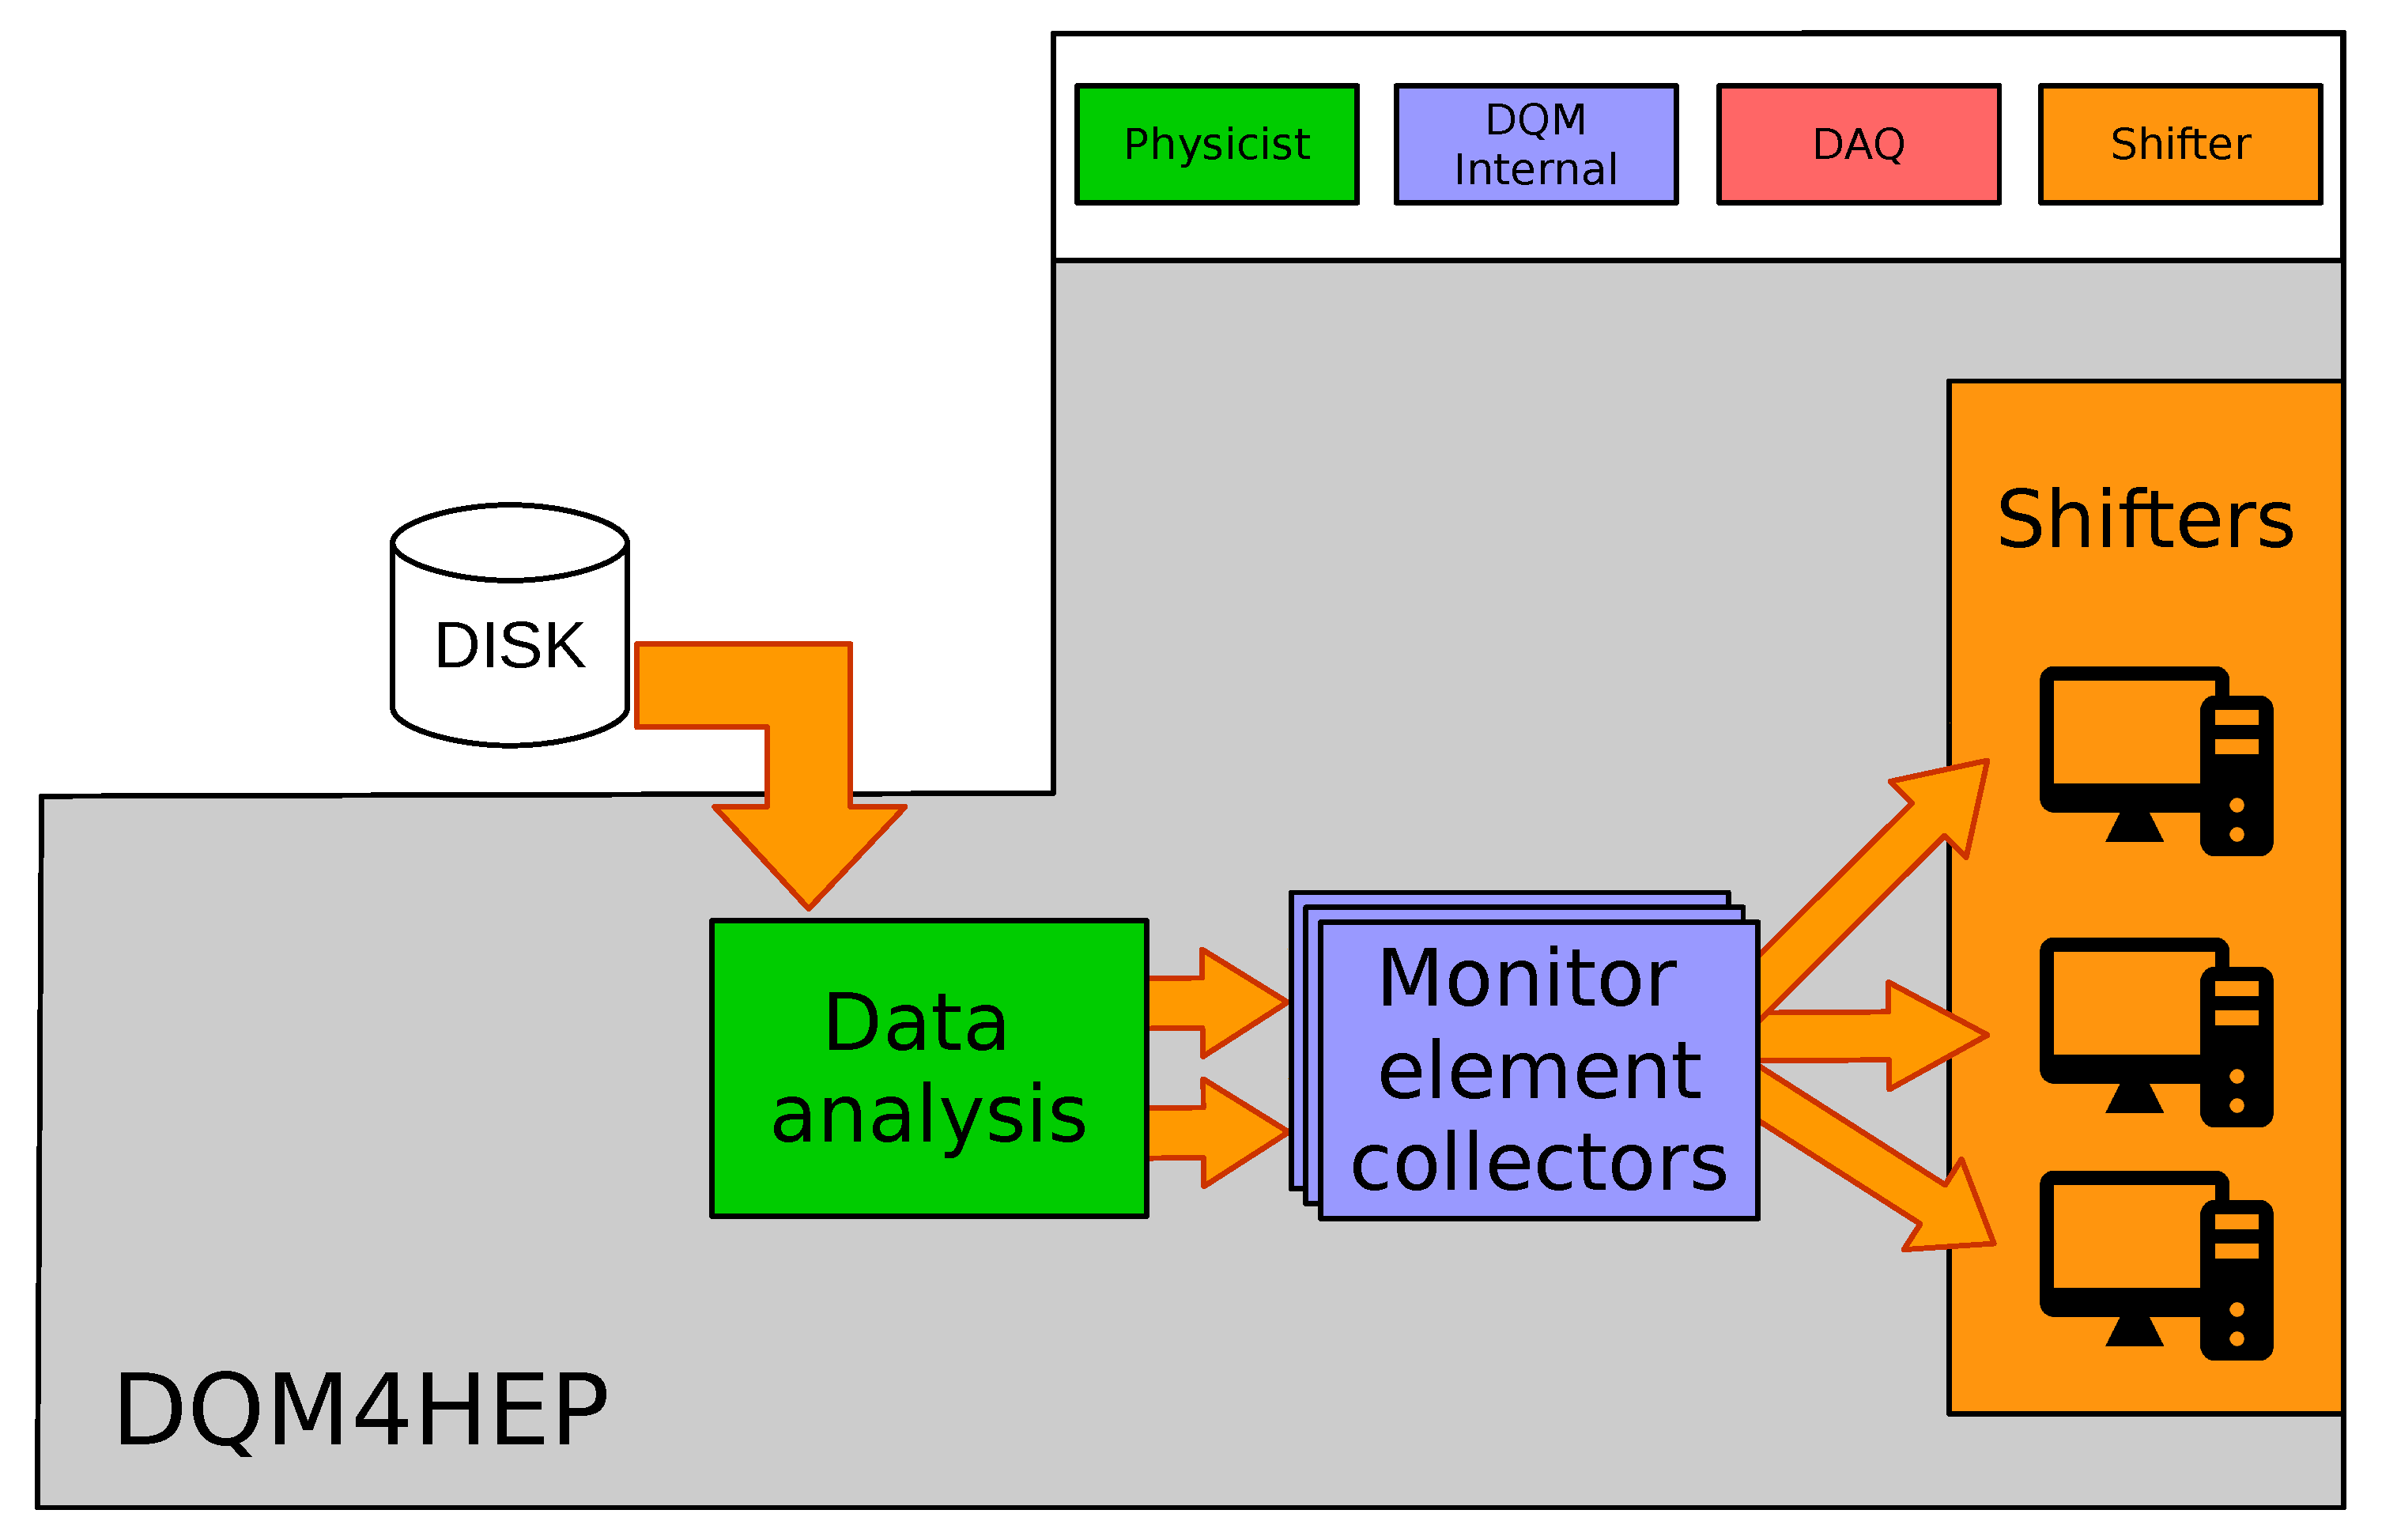
\includegraphics[width=0.95\textwidth]{../Pictures/FileReaderModuleArchitecture.pdf}
	\caption{The structure of running DQM4hep online using a file reader module.}
	\label{figure:daq/dqm4hep/file-reader}
\end{figure}

\subsection{Visualisation and graphical user interface}
As of writing, the graphic user interface and visualisation suite is still under active development. Previous versions of DQM4hep have utilised the Qt framework for GUI and visualisation.

The decision to remove the Qt-based GUI from the framework was made for two reasons. Firstly because of integration with ROOT -- running DQM4hep with a Qt-based GUI requires an installation of ROOT compiled with the \texttt{--enable-Qt} flag enabled, and the majority of ROOT installations in remotely-accsible file systems based at CERN and DESY (which are heavily used for analysis and testbeams) were not compiled this way. Secondly, Qt was an additional dependency that must be installed prior to use, making the software more dependent upon the operating system and environment of the machine, and thus less generic and easy to use.

However, the removal of the Qt-based UI however allows for greater freedom with UI development. The intended goal is to have a browser-based GUI, removing dependency on specific software frameworks, allowing it to function on any device. This will also make it more compact and portable, as the interfaces for run control, networking, and data monitoring and quality display can be simply run in different tabs of the same browser window.

An example of the older Qt-based monitoring GUI in use can  be seen in Fig. \ref{figure:daq/dqm4hep/old-gui}. A mock-up of the web interface can be seen in Fig. \ref{figure:daq/dqm4hep/future-gui}.

\begin{figure}
	\centering
	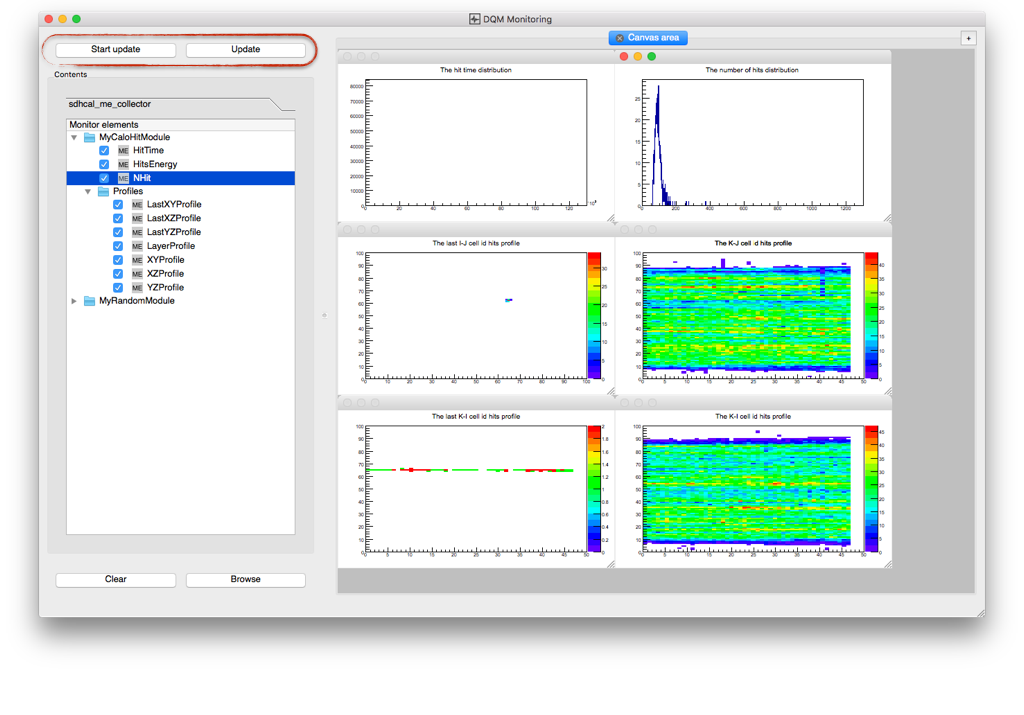
\includegraphics[width=1.0\textwidth]{../Pictures/DQM4hepMonitoringGui.png}
	\caption{An example of the current Qt-based monitoring GUI in use.}
	\label{figure:daq/dqm4hep/old-gui}
\end{figure}

\begin{figure}
	\centering
	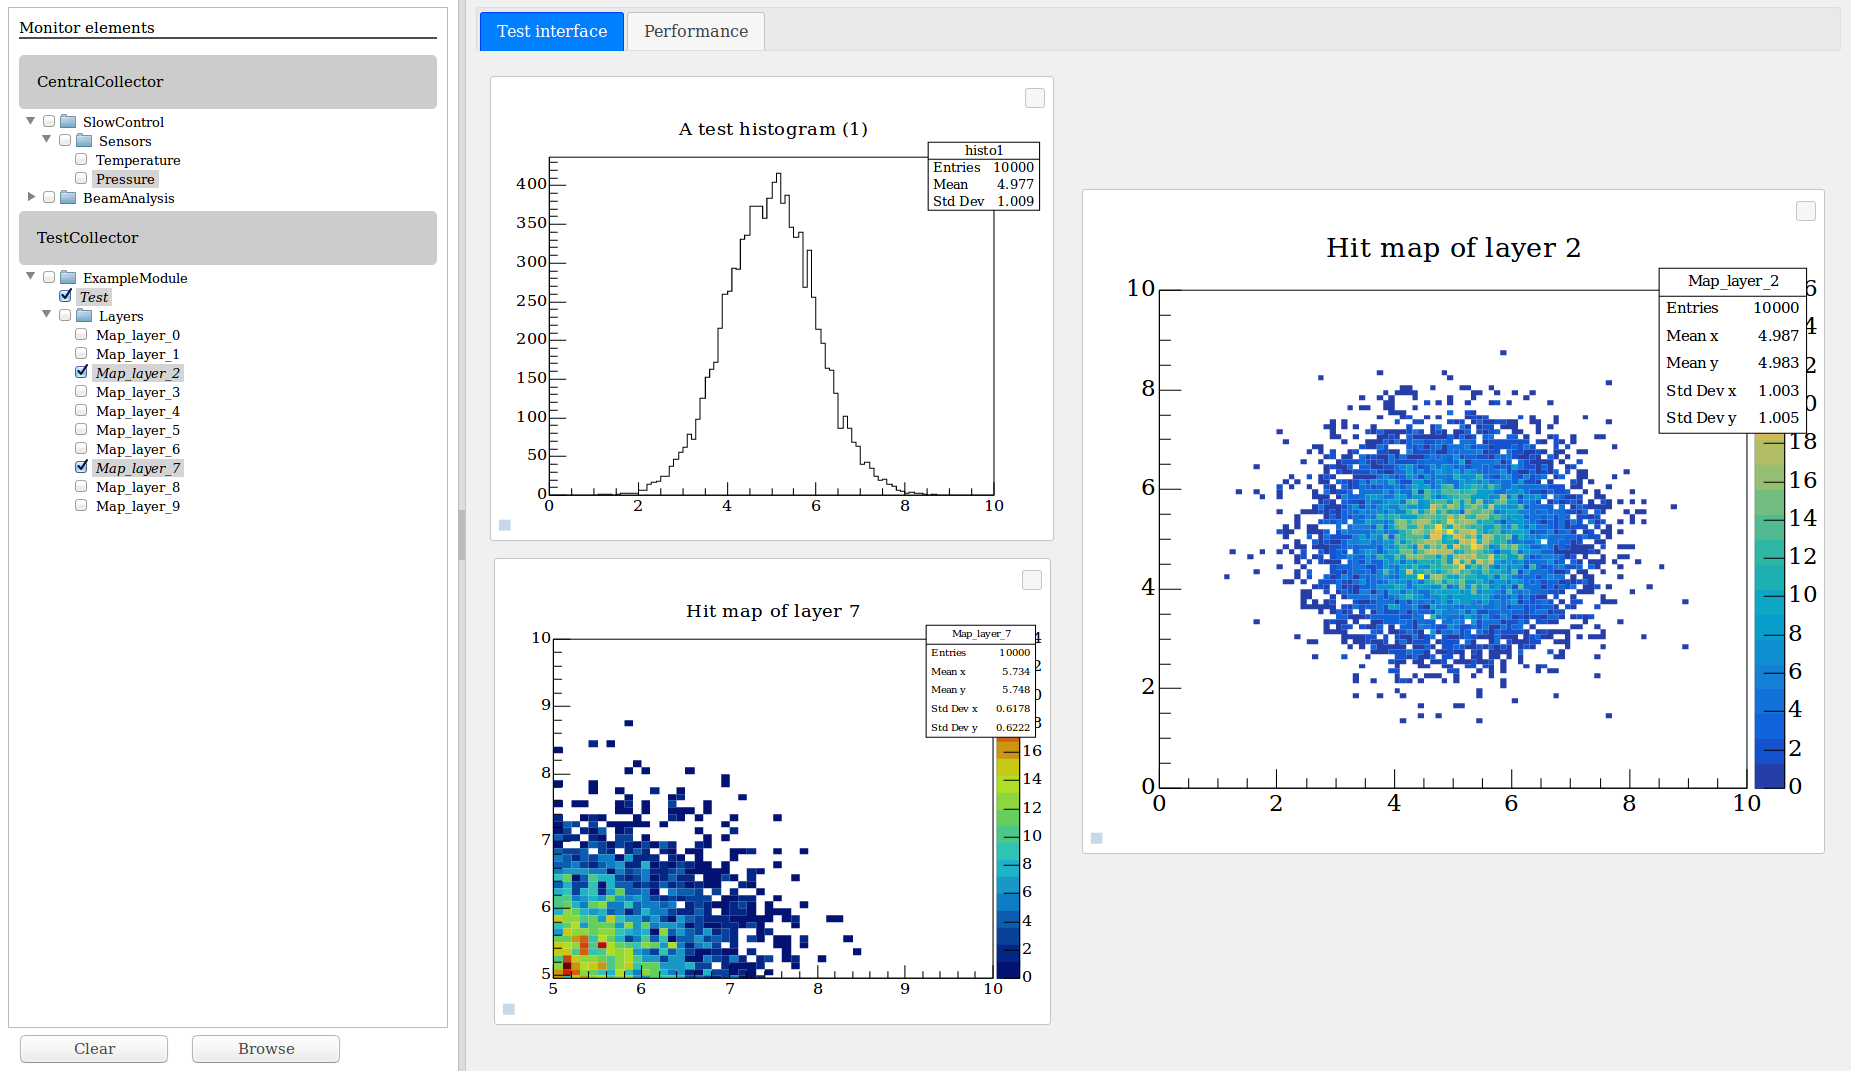
\includegraphics[width=1.0\textwidth]{../Pictures/ScreenshotWebMonitoring.png}
	\caption{A preview of the planned web-based monitoring interface.}
	\label{figure:daq/dqm4hep/future-gui}
\end{figure}

\section{Data quality testing}
One of the important areas of DQM4hep that was not yet completed was data quality monitoring, which is an array of tests or programs that assess the data being taken in real time to allow testbeam operators and shifters without detailed knowledge of the hardware, software, or physics to determine whether the device under test is performing as intended, and to quickly identify and address any errors or inconsistencies. Data quality monitoring (DQM) uses a variety of methods for measuring the `quality' or `goodness' of data, mainly relying upon statistical or comparative methods.

DQM4hep did not have any infrastructure to support data quality tests, but this was added during refactoring for the next release version. Once this was in place, a variety of data quality tests were developed and implemented, detailed below.

\subsection{Property within expected test}
This is a quality test that takes either a TH1 or TGraph object, and finds some user-defined parameter. The parameter must be one of: mean, mean90, root mean square (RMS), root mean square 90 (RMS90), or median. It then checks whether either: that this parameter is within a user-specified range; or that it is above or below the user-specified threshold. If a range is being used, the result is the p-value of the property being within the specified range. If a threshold is being used, then the result is 1 if the property passes the threshold, 0 otherwise.

\subsection{Exact reference comparison test}
This is a quality test that takes any TObject, and compares it to a user-specified reference object (which must be of the same type). The result is 1 if the two objects are identical, 0 otherwise. 

\subsection{Fit parameter in range test}
This is a quality test that takes either a TH1, TGraph, or TGraph2D object and plots a user-defined function onto it, solving for one of the parameters of the function, then checks it against a user-defined range. The result is the p-value of the parameter being within the specified range.

\subsection{Kolmogorov-Smirnov test}
This is a quality test that takes either a TH1 or a TGraph object, and performs the Kolmogorov-Smirnov test between that object and a specified reference. The result is the p-value of the Kolmogorov-Smirnov test. The Kolmogorov-Smirnov test is intended for unbinned data, not histograms, but ROOT provides a function for performing the Kolmogorov-Smirnov test on histograms, so this is functionlity is also included for the sake of completeness.

\subsection{$\chi^2$ test}
This is a quality test that takes a TH1 object and performs the Pearson $\chi^2$ test between that object and a specified reference. This test is analogous to the Kolmogorov-Smirnov test, but is designed specifically to work for binned histogram data. The result is the p-value output by the $\chi^2$ test. 

%\section{Integration with EUDAQ}

\section{Adaptation to other detectors}
Due to the modularity and genericity of DQM4hep, the process of deploying it for a new detector is simple -- the only parts of DQM4hep that need to be made for any specific use case are the analysis modules, standalone modules, streamer plugin, and file reader plugin. For all of these plugins, there are templates available in the codebase, as well as examples of in-use plugins for other detectors. A few special DQM4hep-specific functions are necessary for these plugins to hook into the framework properly, but apart from these all user-provided plugins are written in normal C++ code that also integrates ROOT, so should be familiar to most users.

A file streamer or file reader must be written by the user, given a specific data structure. This requires knowledge of both the event data model of the data acquisition setup, as well as the structure of the data files. The ideal person to write this code is someone with detailed knowledge of the data acquisition software being used, and the data storage or streaming. 

In general, only one of the file streamer or file reader plugins will be needed. If the data will be monitored offline or ``nearly-online'' by loading files from disk, then a file reader plugin must be written. If the data is to be monitored online, then a streamer plugin must be written. Both of these plugins are similar in structure and differ only on where they get the data from -- a file reader loads a file from disk, whereas a streamer loads it from the data acquisition system. 

Once the information is accessible from either the file reader or streamer, the framework handles passing this data to the analysis modules. Analysis modules are a type of plugin which take data that has been packaged into events by a file reader or streamer plugin and performs some analysis on it. This usually takes the form of processing the data in histograms, graphs, or some other plot, but can also include an arbitrary amount of other processing, such as checking validation bits, thresholds, error-checking, and so on. Monitoring the data quality can also be done from within analysis modules, but this is not recommended as dedicated quality tests are available.

% Maybe have an example file reader here, well-commented?

For each analysis module that is being run, an XML steering file is required to provide the parameters and networking information to all the processes needed. A single steering file can call only a single analysis or standalone module, but multiple steering files can be run in parallel by the framework.

Examples of using DQM4hep with testbeams both within the AIDA-2020 community and outside of it can be found in Chapters \ref{chapter:aidatestbeams} and \ref{chapter:ideatestbeam}, respectively.

\section{Documentation and user manual}
One of the biggest hurdles to promoting a new framework is the lack of understanding of it's installation, deployment, and usage. Many research teams will continue to use their existing software solutions, which may be suboptimal or difficult to use, according to the principle of ``better the devil you know than the devil you don't''. The first step to overcoming this is to produce clear, readable and complete documentation across the entire range of features the framework has.

To this end, DQM4hep has two sets of documentation: a Doxygen webite and a user manual.

Many particle physics software frameworks provide documentation in the form of Doxygen, a documentation generator tool. Doxygen is extremely useful, as the documentation for functions and objects is written within the code itself, ensuring that documentation is written as the code is written. Doxygen also automatically compiles a documentation guide using HTML, automatically listing the relationships between objects, structures, functions, etc. that can be compiled and viewed locally, or hosted on the internet as a reference.

One limitation with Doxygen documentation is that is not holistic. Doxygen relies upon the structures of the code, not the program as a whole. Doxygen is extremely useful for developers, as well as already-experienced users, but doesn't aid new users in learning to use a piece of software. Provide this more holistic documentation is very important, and would need to take the form of guides and walkthroughs for common procedures, intended for \emph{users} of the framework with little to no interest in the mechanics of it.

To this end, DQM4hep also has a user manual, compiled using Read the Docs, which provides explanations and worked examples of individual components of the framework and running it as a whole. It also includes instructions and details on how to write plugins of all kinds, and how to run the framework both online and offline. 

The user manual can be found here\cite{dqm4hep-user-manual}, and the Doxygen can be found here\cite{dqm4hep-doxygen}.